\documentclass[14pt, a4paper]{extarticle}
\usepackage[utf8]{inputenc}  % Vietnamese input

\usepackage{hyperref}       % For hypertext inserting
\usepackage{fancyhdr}       % For header and footer
\usepackage{float}          % Force figure placement

\usepackage{niceframe}      % For titlepage
\usepackage{tikz}           % titlepage border
\usetikzlibrary{calc}       % titlepage border
\usepackage{bm}             % \bm for bold text in math

%table padding
\usepackage{array}
\setlength\extrarowheight{2pt} % or whatever amount is appropriate
% table padding

% For tree file structure
\usepackage[edges]{forest}

\definecolor{foldercolor}{RGB}{124,166,198}

\tikzset{pics/folder/.style={code={%
    \node[inner sep=0pt, minimum size=#1](-foldericon){};
    \node[folder style, inner sep=0pt, minimum width=0.3*#1, minimum height=0.6*#1, above right, xshift=0.05*#1] at (-foldericon.west){};
    \node[folder style, inner sep=0pt, minimum size=#1] at (-foldericon.center){};}
    },
    pics/folder/.default={20pt},
    folder style/.style={draw=foldercolor!80!black,top color=foldercolor!40,bottom color=foldercolor}
}

\forestset{is file/.style={edge path'/.expanded={%
        ([xshift=\forestregister{folder indent}]!u.parent anchor) |- (.child anchor)},
        inner sep=1pt},
    this folder size/.style={edge path'/.expanded={%
        ([xshift=\forestregister{folder indent}]!u.parent anchor) |- (.child anchor) pic[solid]{folder=#1}}, inner ysep=0.6*#1},
    folder tree indent/.style={before computing xy={l=#1}},
    folder icons/.style={folder, this folder size=#1, folder tree indent=3*#1},
    folder icons/.default={12pt},
}
% For tree file structure

% Page config
\usepackage[a4paper, left=1.75cm,right=1.75cm,top=2cm,bottom=2cm]{geometry}

% Font config
\usepackage{fontspec}
\setmainfont{SegoeUI}
% Font config

%For code presentation
\usepackage{listings}
\usepackage{color}

\definecolor{bluekeywords}{rgb}{0.13,0.13,1}
\definecolor{greencomments}{rgb}{0,0.5,0}
\definecolor{redstrings}{rgb}{0.9,0,0}

\lstset{
    frame=tb,
    language=[Sharp]C,
    showspaces=false,
    showtabs=false,
    breaklines=true,
    escapeinside={(*@}{@*)},
    commentstyle=\color{greencomments},
    keywordstyle=\color{bluekeywords}\bfseries,
    stringstyle=\color{redstrings},
    basicstyle=\ttfamily,
    aboveskip=3mm,
    belowskip=3mm,
    showstringspaces=false,
    columns=flexible,
    basicstyle={\small\ttfamily},
    numbers=none,
    numberstyle=\tiny\color{gray},
    breaklines=true,
    breakatwhitespace=true,
    tabsize=3
}

\newcommand{\code}[1]{\lstinline[language=[Sharp]C, basicstyle=\color{orange!40!black}\large\ttfamily,
keywordstyle=\color{blue},
commentstyle=\color{green!50!black},]{#1}}

\newcommand{\shell}[1]{\lstinline[language=bash, basicstyle=\color{orange!40!black}\large\ttfamily,
keywordstyle=\color{blue},
commentstyle=\color{green!50!black},]{#1}}
% For code presentation

%For fixed table postition
\usepackage{float}

%For section size
\usepackage{titlesec}

\titleformat*{\section}{\Large\bfseries}
\titleformat*{\subsection}{\Large\bfseries}
\titleformat*{\subsubsection}{\large\bfseries}

\begin{document}
\begin{titlepage}
    \begin{tikzpicture}[remember picture,overlay,inner sep=0,outer sep=0]
        \draw[blue!70!black,line width=4pt] ([xshift=-1.5cm,yshift=-2cm]current page.north east) coordinate (A)--([xshift=1.5cm,yshift=-2cm]current page.north west) coordinate(B)--([xshift=1.5cm,yshift=2cm]current page.south west) coordinate (C)--([xshift=-1.5cm,yshift=2cm]current page.south east) coordinate(D)--cycle;

        \draw ([yshift=0.5cm,xshift=-0.5cm]A)-- ([yshift=0.5cm,xshift=0.5cm]B)--
        ([yshift=-0.5cm,xshift=0.5cm]B) --([yshift=-0.5cm,xshift=-0.5cm]B)--([yshift=0.5cm,xshift=-0.5cm]C)--([yshift=0.5cm,xshift=0.5cm]C)--([yshift=-0.5cm,xshift=0.5cm]C)-- ([yshift=-0.5cm,xshift=-0.5cm]D)--([yshift=0.5cm,xshift=-0.5cm]D)--([yshift=0.5cm,xshift=0.5cm]D)--([yshift=-0.5cm,xshift=0.5cm]A)--([yshift=-0.5cm,xshift=-0.5cm]A)--([yshift=0.5cm,xshift=-0.5cm]A);


        \draw ([yshift=-0.3cm,xshift=0.3cm]A)-- ([yshift=-0.3cm,xshift=-0.3cm]B)--
        ([yshift=0.3cm,xshift=-0.3cm]B) --([yshift=0.3cm,xshift=0.3cm]B)--([yshift=-0.3cm,xshift=0.3cm]C)--([yshift=-0.3cm,xshift=-0.3cm]C)--([yshift=0.3cm,xshift=-0.3cm]C)-- ([yshift=0.3cm,xshift=0.3cm]D)--([yshift=-0.3cm,xshift=0.3cm]D)--([yshift=-0.3cm,xshift=-0.3cm]D)--([yshift=0.3cm,xshift=-0.3cm]A)--([yshift=0.3cm,xshift=0.3cm]A)--([yshift=-0.3cm,xshift=0.3cm]A);

    \end{tikzpicture}



    \centerline{\large{\textbf{ĐẠI HỌC KHOA HỌC TỰ NHIÊN}}}
    \bigskip
    \centerline{\large{ĐẠI HỌC QUỐC GIA THÀNH PHỐ HỒ CHÍ MINH}}

    \centerline{\Large{--------------------------------------}}

    \bigskip

    \centerline{
\includegraphics[width=40mm]{logo.jpg}}

    \centerline{\niceframe[14cm]
        {
            \begin{center}
                \LARGE{\textbf{ĐỒ ÁN THỰC HÀNH 1}}
                \linebreak
                \centering\LARGE{\textbf{LẬP TRÌNH SOCKET}}
            \end{center}
        }
    }

    \bigskip
    \bigskip

    \centerline{\LARGE{\textbf{Mạng máy tính}}}
    \raggedright
    \bigskip
    \medskip
    \begin{center}

        \begin{table}[h]
            \begin{tabular}{rrlc}
                 & Giảng viên lý thuyết & Lê Ngọc Sơn       &          \\
                 & Trợ giảng            & Lê Hà Minh        &          \\
                 & Giảng viên thực hành & Nguyễn Thanh Quân &          \\
                 &                &                   &          \\
                 &                & Phù Thành Nhân    & 21127382 \\
                 &                & Võ Thanh Tú       & 21127469 \\
                 &                & Nguyễn Quốc Huy   & 21127511
            \end{tabular}
        \end{table}
        \LARGE{21CLC02}
    \end{center}
\end{titlepage}

%Header&Footer

\pagestyle{fancy}
\fancyhf{}
\addtolength{\topmargin}{-0.70894pt}
\setlength{\headheight}{12.70894pt}

\setlength{\parindent}{0cm}     % prevent indent
\lhead{\textbf{FIT-HCMUS}}
\rhead{\textbf{Mạng máy tính}}
\rfoot{\textbf{\thepage}}

%rename content table
\renewcommand*{\contentsname}{Mục lục}
\renewcommand*{\figurename}{Hình}
\tableofcontents
\newpage
\section{Đánh giá mức độ hoàn thành}
\begin{table}[h!]
    \centering
    \begin{tabular}{| p{0.05\linewidth}| p{0.3\linewidth}| p{0.35\linewidth}| p{0.20\linewidth}|}
        \hline
        \textbf{STT}                & \textbf{Chức năng}                & \textbf{Ý nghĩa}                & \textbf{Mức độ hoàn thành} \\
        \hline
        1                & \textbf{KẾT NỐI}                  & \textbf{0.5 điểm}                  & 100\%                \\
                   &                  & Cho phép client kết nối đến server thông qua kết nối TCP                     &                \\
        \hline
        2                & \textbf{QUẢN LÝ KẾT NỐI}          & \textbf{0.5 điểm}                  & 100\%                \\
                   &                  & Khi client hoặc server mất kết nối đột ngột, không làm chương trình treo hay xảy ra lỗi             &                \\
        \hline
        3                & \textbf{Tải được page index.html} & \textbf{3.5 điểm}                  & 100\%                \\
                   &                  & Browser có thể render lên đầy đủ nội dung của trang index.html.                    &                \\
                   &                  &
        Trang index.html hiển thị 1 HTML form cho phép đăng nhập (yêu cầu 4). &                     \\
        \hline
        4                & \textbf{ĐĂNG NHẬP}                & \textbf{2 điểm}                 & 100\%                \\
                   &                  & \textbf{POST} method, gửi \textbf{"uname"} là \textbf{"admin} và \textbf{"psw"} là \textbf{"123456} &                \\
        \hline
        5                & \textbf{LỖI PAGE}                 & \textbf{0.5 điểm}                  & 100\%                \\
                   &                  & Trả 404 khi load page không đúng                 &                \\
        \hline
        6                & \textbf{MULTIPLE CONNECTIONS}     & \textbf{1 điểm}                 & 100\%                \\
                   &                  & Concurrent, handle nhiều client cùng lúc                  &                \\
        \hline
        7                & \textbf{REPORT}                   & \textbf{1 điểm}                 & 100\%                \\
                   &                  & Theo quy định                   &                \\
        \hline
    \end{tabular}
\end{table}
\section{Kịch bản giao tiếp của chương trình}
\subsection{Giao thức trao đổi}
\begin{itemize}
    \item Phần mềm sử dụng giao thức HTTP làm giao thức truyền thông chính. HTTP là từ viết tắt của \textbf{Hyper Text Transfer Protocol} nghĩa là \textbf{Giao thức Truyền tải Siêu Văn Bản}, là nền tảng truyền thông của World Wide Web.
    \item Browser tạo kết nối TCP/IP đến WebServer, gửi một HTTP request cho máy chủ thông qua kết nối đó, đọc kết quả trả về (HTTP response) và hiển thị nội dung trang web (page) cho người dùng.
\end{itemize}
\subsection{Cấu trúc thông điệp}

Mỗi thông điệp HTTP được chia làm 2 loại chính là Request (chỉ nhận 1 Response phản hồi lại) và Response(chỉ phản hồi cho 1 Request). Chúng gồm 3 thành phần chính:
\begin{itemize}
    \item Dòng đầu tiên của thông điệp, được gọi là \textbf{Start Line} trong \textit{HTTP Request}, hoặc \textbf{Status Line} trong \textit{HTTP Response}. Dòng này sẽ định nghĩa loại yêu cầu request đến Server và loại phản hồi của response từ server cho request trước đó.
    \item Phần tiếp theo, được ngăn cách với phần đầu tiên bới chuỗi ký tự xuống dòng "$\bm{\backslash r \backslash n}$", chính là \textbf{Headers}. Những trường header này còn được chia thành 2 loại là \textbf{General Headers} và \textbf{Request Headers/Response Headers}. Mỗi header là 1 cặp key, value được ngăn cách bởi dấu hai chấm (:), không phân biệt hoa thường. Các header sẽ được ngăn cách với nhau bằng chuỗi ký tự xuống dòng. Các header này sẽ bổ trợ nội dung cần thiết cho request và response. Tại header cuối cùng, phần header sẽ được kết thúc bằng 1 dòng trống (nghĩa là sẽ xuất hiện chuỗi "$\bm{\backslash r \backslash n}\bm{\backslash r \backslash n}$"
    )
    \item Phần cuối cùng là phần \textbf{Data}. Phần này là 1 phần không bắt buộc, nó chỉ xuất hiện khi Request hoặc Response có nhu cầu gửi kèm theo dữ liệu đến đích.
\end{itemize}
\subsection{Kiểu dữ liệu của thông điệp}

HTTP Message Start Line, Status Line và Headers là những đoạn văn bản được mã hoá bằng bộ mã ASCII, còn phần Data của thông điệp sẽ là dạng byte hoặc dạng văn bản (kiểu mã hoá sẽ được quy định tại header \textit{Content-Type}, mặc định là mã hoá bằng bộ mã ASCII)
\subsection{Cách tổ chức cơ sở dữ liệu}

Do việc tổ chức cơ sở dữ liệu không phải mục tiêu chính của môn học nên nhóm quyết định sẽ lưu dữ liệu dưới dạng 1 file \textit{.txt} đơn giản được mã hoá bằng ASCII, không có mã hoá bảo mật. 
\section{Hướng dẫn sử dụng}
\subsection{Các cách khởi động chương trình}

Chương trình được phát hành đến người dùng dưới dạng file thực thi cho hệ điều hành Windows ($NetworkSocket.exe$) Để khởi động chương trình, người dùng có 2 cách:
\begin{enumerate}
    \item Dùng môi trường dòng lệnh, dùng câu lệnh và các option được đề cập ở mục bên dưới.
    \item Nháy đúp chuột vào file thực thi ($.exe$) của chương trình
\end{enumerate}
\begin{figure}[!h]
    \begin{center}
        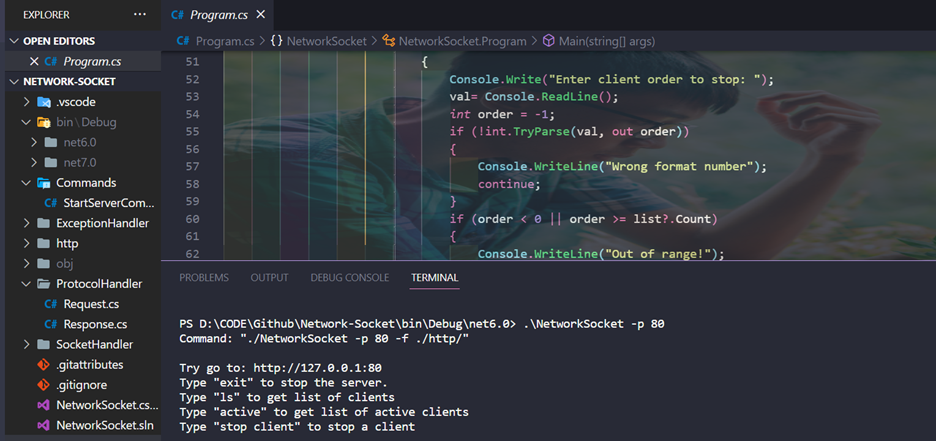
\includegraphics{PicGuide/Start.png}
        \caption{Mở chương trình bằng Terminal tích hợp trong phần mềm VSCode}
    \end{center}
\end{figure}
\subsection{Các tuỳ chỉnh cho Chương trình dòng lệnh (CLI)}

Với tên chương trình là $NetworkSocket.exe$, trình dòng lệnh mẫu là $Windows PowerShell$\\

Để chạy chương trình, ta dùng lệnh\\
\begin{center}
    \shell{./NetworkSocket.exe}
\end{center}
Khi dùng dòng lệnh, nếu thêm các flag sau thì người dùng có thể tuỳ chỉnh được chương trình trước khi khởi động:
\begin{figure}[!h]
    \begin{center}
        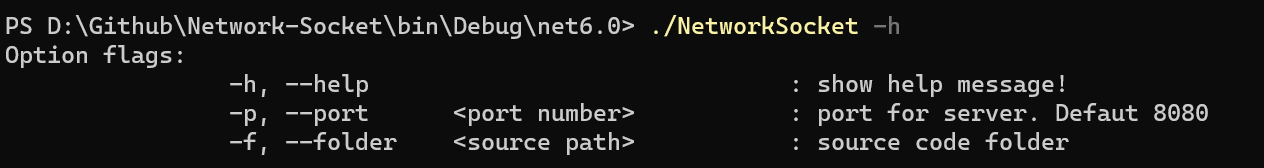
\includegraphics{PicGuide/Help.png}
        \caption{Gọi lệnh \shell{./NetworkSocket.exe -h}}
    \end{center}
\end{figure}
\begin{itemize}
    \item Flag \textbf{-h} giúp hiển thị thông tin các flag
    \item Flag \textbf{-p} giúp chọn port phần mềm sẽ bắt đầu, mặc định là \textit{8080}
    \item Flag \textbf{-f} giúp chọn thư mục chứa mã nguồn trang web, mặc định là thư mục \textit{http} của chương trình
\end{itemize}
\subsection{Các tuỳ chỉnh còn lại}

Sau khi khởi động, menu sẽ hiển thị lên các lệnh đã được thêm vào giúp người dùng thao tác nhanh.
Bạn có thể nhấp vào dòng chữ \href{http://127.0.0.1:8080}{http://127.0.0.1:8080} sẽ dẫn tới trang web trên trình duyệt. Đường dẫn này sẽ thay đổi tuỳ theo cài đặt port hiện tại của chương trình.\\

Và những lệnh khác tương ứng với hướng dẫn đi kèm, các lệnh này được thực thi trong suốt chương trình. Nếu bạn muốn dừng server chỉ cần nhập \shell{exit} server sẽ ngừng ở mọi thời điểm.\\

Lưu ý rằng các câu lệnh sẽ không phân biệt hoa thường\\

Khi mở client trên trình duyệt sẽ hiện các nội dung được gửi về như sau\\
\begin{figure}[H]
    \begin{center}
        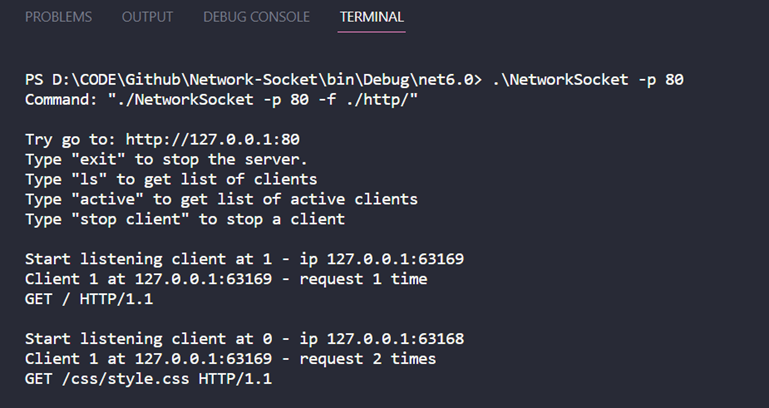
\includegraphics{PicGuide/Success.png}
        \caption{Các hoạt động gửi nhận thông điệp}
    \end{center}
\end{figure}
Khi sử dụng lệnh \shell{ls}\\
\begin{figure}[H]
    \begin{center}
        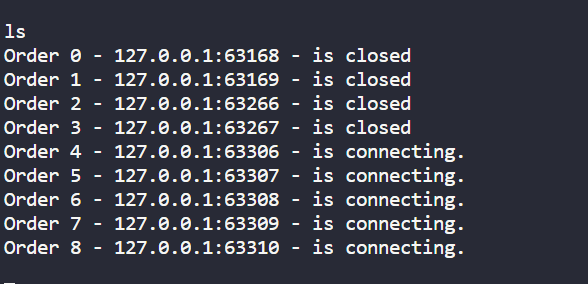
\includegraphics{PicGuide/LS.png}
        \caption{Số lượng client đã kết nối kể cả các client bị đóng.}
    \end{center}
\end{figure}
Khi nhập lệnh \shell{stop client}, menu sẽ yêu cầu nhập thứ tự client mà bạn muốn đóng\\
\begin{figure}[H]
    \begin{center}
        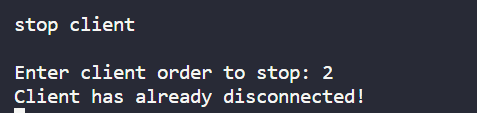
\includegraphics{PicGuide/Stop Client.png}
        \caption{Lệnh đóng kết nối đến 1 client}
    \end{center}
\end{figure}

Khi nhập lệnh \shell{active}, hệ thống sẽ cho biết có bao nhiêu client đang được kết nối
\begin{figure}[H]
    \begin{center}
        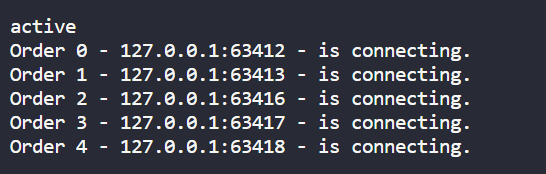
\includegraphics{PicGuide/Active.png}
        \caption{Kiểm tra các kết nối đang hoạt động}
    \end{center}
\end{figure}
Khi nhập lệnh shell{exit}, hệ thống sẽ dừng kết nối tất cả các client đang kết nối và kết thúc chương trình.
\begin{figure}[H]
    \begin{center}
        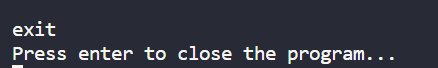
\includegraphics{PicGuide/Exit.png}
        \caption{Kết thúc chương trình}
    \end{center}
\end{figure}
\section{Môi trường lập trình và framework hỗ trợ}
\begin{itemize}
    \item Hệ điều hành sử dụng chính: Windows 10, Windows 11
    \item Ngôn ngữ sử dụng: C\# 10.0
    \item Nền tảng lập trình: .NET 6.0
    \item IDE: Visual Studio 2022 Community
\end{itemize}
\section {Cấu trúc mã nguồn}
\begin{center}
    \begin{forest}
        for tree={
        font=\ttfamily\Large,
        grow'=0,
        folder indent=.9em, folder icons,
        edge=densely dotted
        }
        [Network Socket
            [NetworkSocket.csproj, is file]
            [NetworkSocket.sln, is file]
            [Program.cs, is file]
            [Commands
                    [StartServerCommand.cs, is file]
            ]
            [ExceptionHandler
                    [ExceptionResponser.cs, is file]
                    [HelpException.cs, is file]
                    [InvalidCommandException.cs, is file]
            ]
            [http
                    [index.html, is file]
                    [..., is file]
            ]
            [ProtocolHandler
                    [HttpProtocol.cs, is file]
                    [Request.cs, is file]
                    [Response.cs, is file]
                    [RequestHandler.cs, is file]
            ]
            [SocketHandler
                    [HTTPClient.cs, is file]
                    [Server.cs, is file]
            ]
            [User
                    [UserDataContext.cs, is file]
                    [UserInfo.cs, is file]
            ]
            [User.txt, is file]
        ]
    \end{forest}
\end{center}
\newpage
\begin{itemize}
    \item \textbf{NetworkSocket.csproj, NetworkSocket.sln:} các file config project, solution của Visual Studio.
    \item \textbf{Program.cs}: file chứa hàm main, nơi chương trình bắt đầu.
    \item Thư mục \textbf{Commands}: các hàm xử lý cài đặt chương trình qua console.
    \begin{itemize}
        \item \textbf{StartServerCommand.cs}: lớp StartServerCommand, dùng để tạo các command cho chương trình.
    \end{itemize}
    \item  Thư mục \textbf{ExceptionHandler} chứa các ngoại lệ (Exception) chưa được định nghĩa nhưng có thể xảy ra trong chương trình.
    \begin{itemize}
        \item \textbf{ExceptionResponser.cs} lớp chịu trách nhiệm chính cho việc xử lý các Exception. Gần như bộ các Exception sẽ được điều hướng về đây.
        \item \textbf{HelpException.cs}: Exception này được gọi khi người dùng nhập sai cú pháp command hoặc khi lệnh help được gọi.
        \item \textbf{InvalidCommandException.cs}: được gọi khi người dùng gọi 1 command không tồn tại.
    \end{itemize}
    \item Thư mục \textbf{http} chứa các thành phần của trang web cần gửi cho client.
    \item Thư mục \textbf{ProtocolHandler} chứa những phần code xử lý HTTP protocol.
    \begin{itemize}
        \item  \textbf{HttpProtocol.cs}: Lớp HttpProtocol, khai báo những thành phần cơ bản cần dùng trong giao thức Http.
        \item \textbf{Request.cs}: Lớp Request kế thừa từ HttpProtocol, sẽ nhận dữ liệu là 1 chuỗi và xây dựng thành 1 đối tượng chứa các thông số của 1 request Http đơn giản.
        \item \textbf{Response.cs}: kế thừa từ HttpProtocol, lớp này chịu trách nhiệm xây dựng response cho các request http đến máy chủ.
        \item \textbf{RequestHandler.cs}: chịu trách nhiệm lựa chọn loại response nào sẽ được dùng và sẽ đính kèm những thông tin gì
    \end{itemize}
    \item Thư mục \textbf{SocketHandler} chứa những phần code xử lý tcp socket.
    \begin{itemize}
        \item \textbf{HTTPClient.cs}: Lớp định nghĩa client chuyên dùng để nhận các đoạn thông điệp Http, sẽ nhận về đối tượng request và dùng lớp RequestHandler để lựa chọn câu trả lời cho client.
        \item \textbf{Server.cs}: Lớp định nghĩa server, chịu trách nhiệm chấp nhận kết nối và tạo các đối tượng HTTPClient tương ứng cho các kết nối đến.
    \end{itemize}
    \item Thư mục \textbf{User}, chứa các lớp quản lý thông tin người dùng.
    \begin{itemize}
        \item \textbf{UserInfo.cs} chứa các thông tin đăng nhập cơ bản của người dùng.
        \item \textbf{UserDataContext.cs} đầu mối liên kết giữa cơ sở dữ liệu người dùng và chương trình. 
    \end{itemize}
    \item \textbf{User.txt} là cơ sở dữ liệu đơn giản dạng file văn bản, lưu trữ thông tin đăng nhập của người dùng.
\end{itemize}

\newpage
\section{Bảng phân công}
\begin{table}[h!]
    \centering
    \begin{tabular}{| p{0.05\linewidth}| p{0.55\linewidth}| p{0.30\linewidth}|}
        \hline
        \textbf{STT} & \textbf{Nhiệm vụ} & \textbf{Người được giao} \\
        \hline
        1   & Viết file \textit{StartServerCommand.cs} & Phù Thành Nhân\\
        \hline
        2   & Viết file \textit{Progam.cs} & Phù Thành Nhân\\
        \hline
        3   & Viết thư mục \textit{ExceptionHandler.cs} & Nguyễn Quốc Huy\\
        \hline
        4   & Viết file \textit{HttpProtocol.cs} & Võ Thanh Tú\\
        5   & Viết file \textit{RequestHandler.cs}      & Võ Thanh Tú\\
        6   & Viết file \textit{Request.cs}     & Nguyễn Quốc Huy\\
        7   & Viết file \textit{Response.cs}    & Nguyễn Quốc Huy\\
        \hline
        8   & Viết file \textit{HTTPClient.cs}  & Nguyễn Quốc Huy\\
        9   & Viết file \textit{Server.cs}      &
        Võ Thanh Tú\\
        \hline
        10  &Viết file \textit{UserInfo.cs}         & Phù Thành Nhân\\
        11  &Viết file \textit{UserDataContext.cs}  & Võ Thanh Tú\\
        \hline
        12  &Tổng hợp báo cáo thành PDF         & Phù Thành Nhân\\
        \hline
    \end{tabular}
\end{table}
\section{Các nguồn tham khảo}
\begin{itemize}
    \item \href{https://tuhocict.com/ky-thuat-lap-trinh-voi-tcp-socket/}{tuhocict.com - Kỹ thuật lập trình TCP socket với C\#}
    \item \href{https://xuanthulab.net/networking-giao-thuc-tcp-voi-cac-lop-tcplistener-tcpclient-va-cac-lop-uri-ipaddress-c-c-sharp.html}{xuanthulab.net - Giao thức TCP trong C\#}
    \item \href{https://xuanthulab.net/lap-trinh-bat-dong-bo-asynchronou-c-c-sharp-voi-bat-dong-bo-theo-mo-hinh-tac-vu.html}{xuanthulab.net - Lập trình bất đồng bộ asynchronou C\# theo Task-base}
    \item \href{https://docs.google.com/document/d/1mjws5-vU9mzq9QgmrwzM3hi9A93vp77mgJK-Cjmy5Cs/edit#heading=h.cfrw1cej12t6}{Hướng dẫn thực hành đồ án 1 - Socket}
    \item \href{https://developer.mozilla.org/en-US/docs/Web/HTTP/Messages}{Mozilla - HTTP Message Structure}
    \item \href{https://vi.wikipedia.org/wiki/Hypertext_Transfer_Protocol}{Wikipedia tiếng Việt - Hypertext Transfer Protocol}
\end{itemize}
\end{document}